\begin{figure}
    \centering
    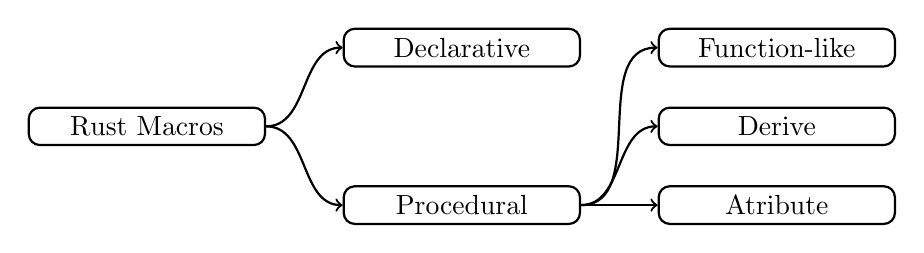
\begin{tikzpicture}
        \tikzset{
            member/.style={
                    rectangle,
                    rounded corners,
                    draw=black,
                    thick,
                    minimum width=3cm,
                },
            connection/.style={->, thick},
        }
        % \draw (0, -2) grid (6, 2);
        \node[member] (root) at (-1, 0) {Rust Macros};
        \node[member] (decl) at (3, 1) {Declarative};
        \node[member] (proc) at (3, -1) {Procedural};
        \node[member] (func) at (7, 1) {Function-like};
        \node[member] (derv) at (7, 0) {Derive};
        \node[member] (attr) at (7, -1) {Atribute};
        \draw[connection] (root) edge[out=0, in=180] (proc);
        \draw[connection] (root) edge[out=0, in=180] (decl);
        \draw[connection] (proc) edge[out=0, in=180] (func);
        \draw[connection] (proc) edge[out=0, in=180] (derv);
        \draw[connection] (proc) edge[out=0, in=180] (attr);
    \end{tikzpicture}
    \caption{Rust macro's family tree}
    \label{fig:rust-macro-family}
\end{figure}